\section{Introduction}
The idea of creating models that can predict output based on some input could be extremely valuable. The models are created by trying to find mathematical relationships in the data so that they can reproduce a desired output. Hopefully, the relationships are generally valid and make the model capable of predicting new unseen data. Models like these could be as simple as regression to the complexity of deep neural networks. The simple models are easy to understand and easy to implement, but their ability to learn complicated relationships can be to somewhat limited. That is why methods such as neural networks and support vector machines have become popular and will be representing our main methods in this project.
\\
\par
Models that are capable of predicting can help humans in decision making, reduce the number of experiments and observations needed and could replace humans in doing boring and repetitive tasks which humans normally are not good at. Or as in this case, reproduce results that allows us to analyze the information behind a certain outcome, such as the presidential election in the United States.  
\\
\par
The bias-variance tradeoff is a fundamental dilemma in statistical learning theory. Bias is erroneous assumptions in a model, so that the model misses out on important relationships. This is called underfitting. Variance is error from sensitivity to fluctuations in the training data. This is called overfitting. Our project will divide the provided data into training and test data, such that this can be observed as well.[1]

\begin{figure}[H]
\centering
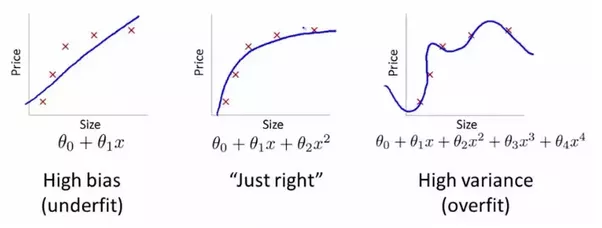
\includegraphics[scale=0.6]{pictures/Bias_variance}
\caption{A simple visual example of underfitting and overfitting.}
\end{figure}

In classification, models are normally assessed based on the percentage of correct calculated labels, which will be used as metric here. 

\begin{equation}
Accuracy = \frac{\sum_{i=1}^n I(t_i=y_i)}{n}
\end{equation}